\documentclass[11pt,a4paper]{article}
\usepackage[utf8]{inputenc}
\usepackage[T1]{fontenc}
\usepackage{geometry}
\geometry{a4paper, margin=1in}
\usepackage{graphicx}
\usepackage{xcolor}
\usepackage{hyperref}
\usepackage{tabularx}
\usepackage{booktabs}
\usepackage{tcolorbox}
\usepackage{amsmath}

\definecolor{primary}{HTML}{0B0F19}
\definecolor{accent}{HTML}{00FF9D}
\definecolor{highlight}{HTML}{FF4F4F}

\hypersetup{
    colorlinks=true,
    linkcolor=blue,
    filecolor=magenta,      
    urlcolor=blue,
    pdftitle={LeanFlow Marketing Prospectus},
}

\begin{document}

\begin{center}
    {\Huge \bfseries BEYOND ``COLORFUL FLUID DYNAMICS''} \\ \vspace{0.5cm}
    {\Large \bfseries Introducing LeanFlow: The World’s First Formally Specified, Cryptographically Sealed CFD Engine} \\ \vspace{0.3cm}
    {\large \textit{Whitepaper \& Product Brief | SocrateAI Research \& DeepMind Science Collaboration}}
\end{center}

\vspace{0.5cm}
\hrule
\vspace{0.5cm}

\section*{The Billion-Dollar Problem with Legacy CFD}

For decades, industries relying on Computational Fluid Dynamics (CFD)---from aerospace and automotive to MedTech and nuclear energy---have accepted a dangerous compromise. Traditional finite-volume solvers (like OpenFOAM) rely heavily on "artificial viscosity" and numerical diffusion to remain mathematically stable. 

When pushed to their limits by coarse meshes, extreme parameters, or boundary conflicts, these legacy solvers do not fail; instead, they silently smooth over mathematical errors, hallucinating plausible but physically impossible results.

\begin{tcolorbox}[colback=red!5!white,colframe=red!75!black,title=WARNING]
In the engineering industry, this is jokingly called \textbf{"Colorful Fluid Dynamics."} But the financial impact is no joke. Millions of dollars are wasted constructing physical prototypes based on flawed simulation data, leading to catastrophic late-stage redesigns and immense regulatory friction.
\end{tcolorbox}

\section*{The LeanFlow Revolution: Trust as an Engineering Asset}

LeanFlow is a dual-scale pseudo-spectral PDE solver that shifts CFD from a "best-effort estimate" to a mathematically certain, legally auditable asset (protected by \textbf{Brevet INPI}).

Coupling a high-precision numerical engine (Lawson IF-RK2 and Streamfunction-Vorticity) with the Lean 4 interactive theorem prover, LeanFlow maps the fundamental laws of physics directly to its code architecture. 

\vspace{0.5cm}
\hrule
\vspace{0.5cm}

\section*{Empirical Proof: LeanFlow vs. Traditional FVM Solvers}

Based on the final benchmark execution data (Cryptographic SHA-256 Seal: \texttt{0ae0e5d97da424e0}), we can objectively evaluate the precise, quantifiable gains of \textbf{LeanFlow} against legacy Computational Fluid Dynamics (CFD) solvers---such as OpenFOAM, ANSYS Fluent, and Star-CCM+.

While traditional Finite Volume (FV) solvers are necessary generalists for handling highly complex, unstructured CAD geometries (e.g., airflow around a complete automobile chassis), they inherently suffer from truncation errors, numerical diffusion, and rely on iterative approximations.

LeanFlow’s dual-scale pseudo-spectral architecture, combined with Lawson IF-RK2/ETD-RK4 time integration and Streamfunction-Vorticity formulations, yields massive computational and epistemic advantages in high-fidelity regimes. Here is the evaluation of LeanFlow's gains versus legacy solvers, grounded \textit{strictly} in the benchmark metrics.

\subsection*{1. The Precision Gain: Zero Numerical Diffusion}

Traditional FV solvers rely on 2nd-order spatial discretization. Computing fluxes across discrete cell boundaries inherently introduces "numerical diffusion"---an algorithmic truncation error that acts as a fake, artificial viscosity.

\begin{figure}[h]
    \centering
    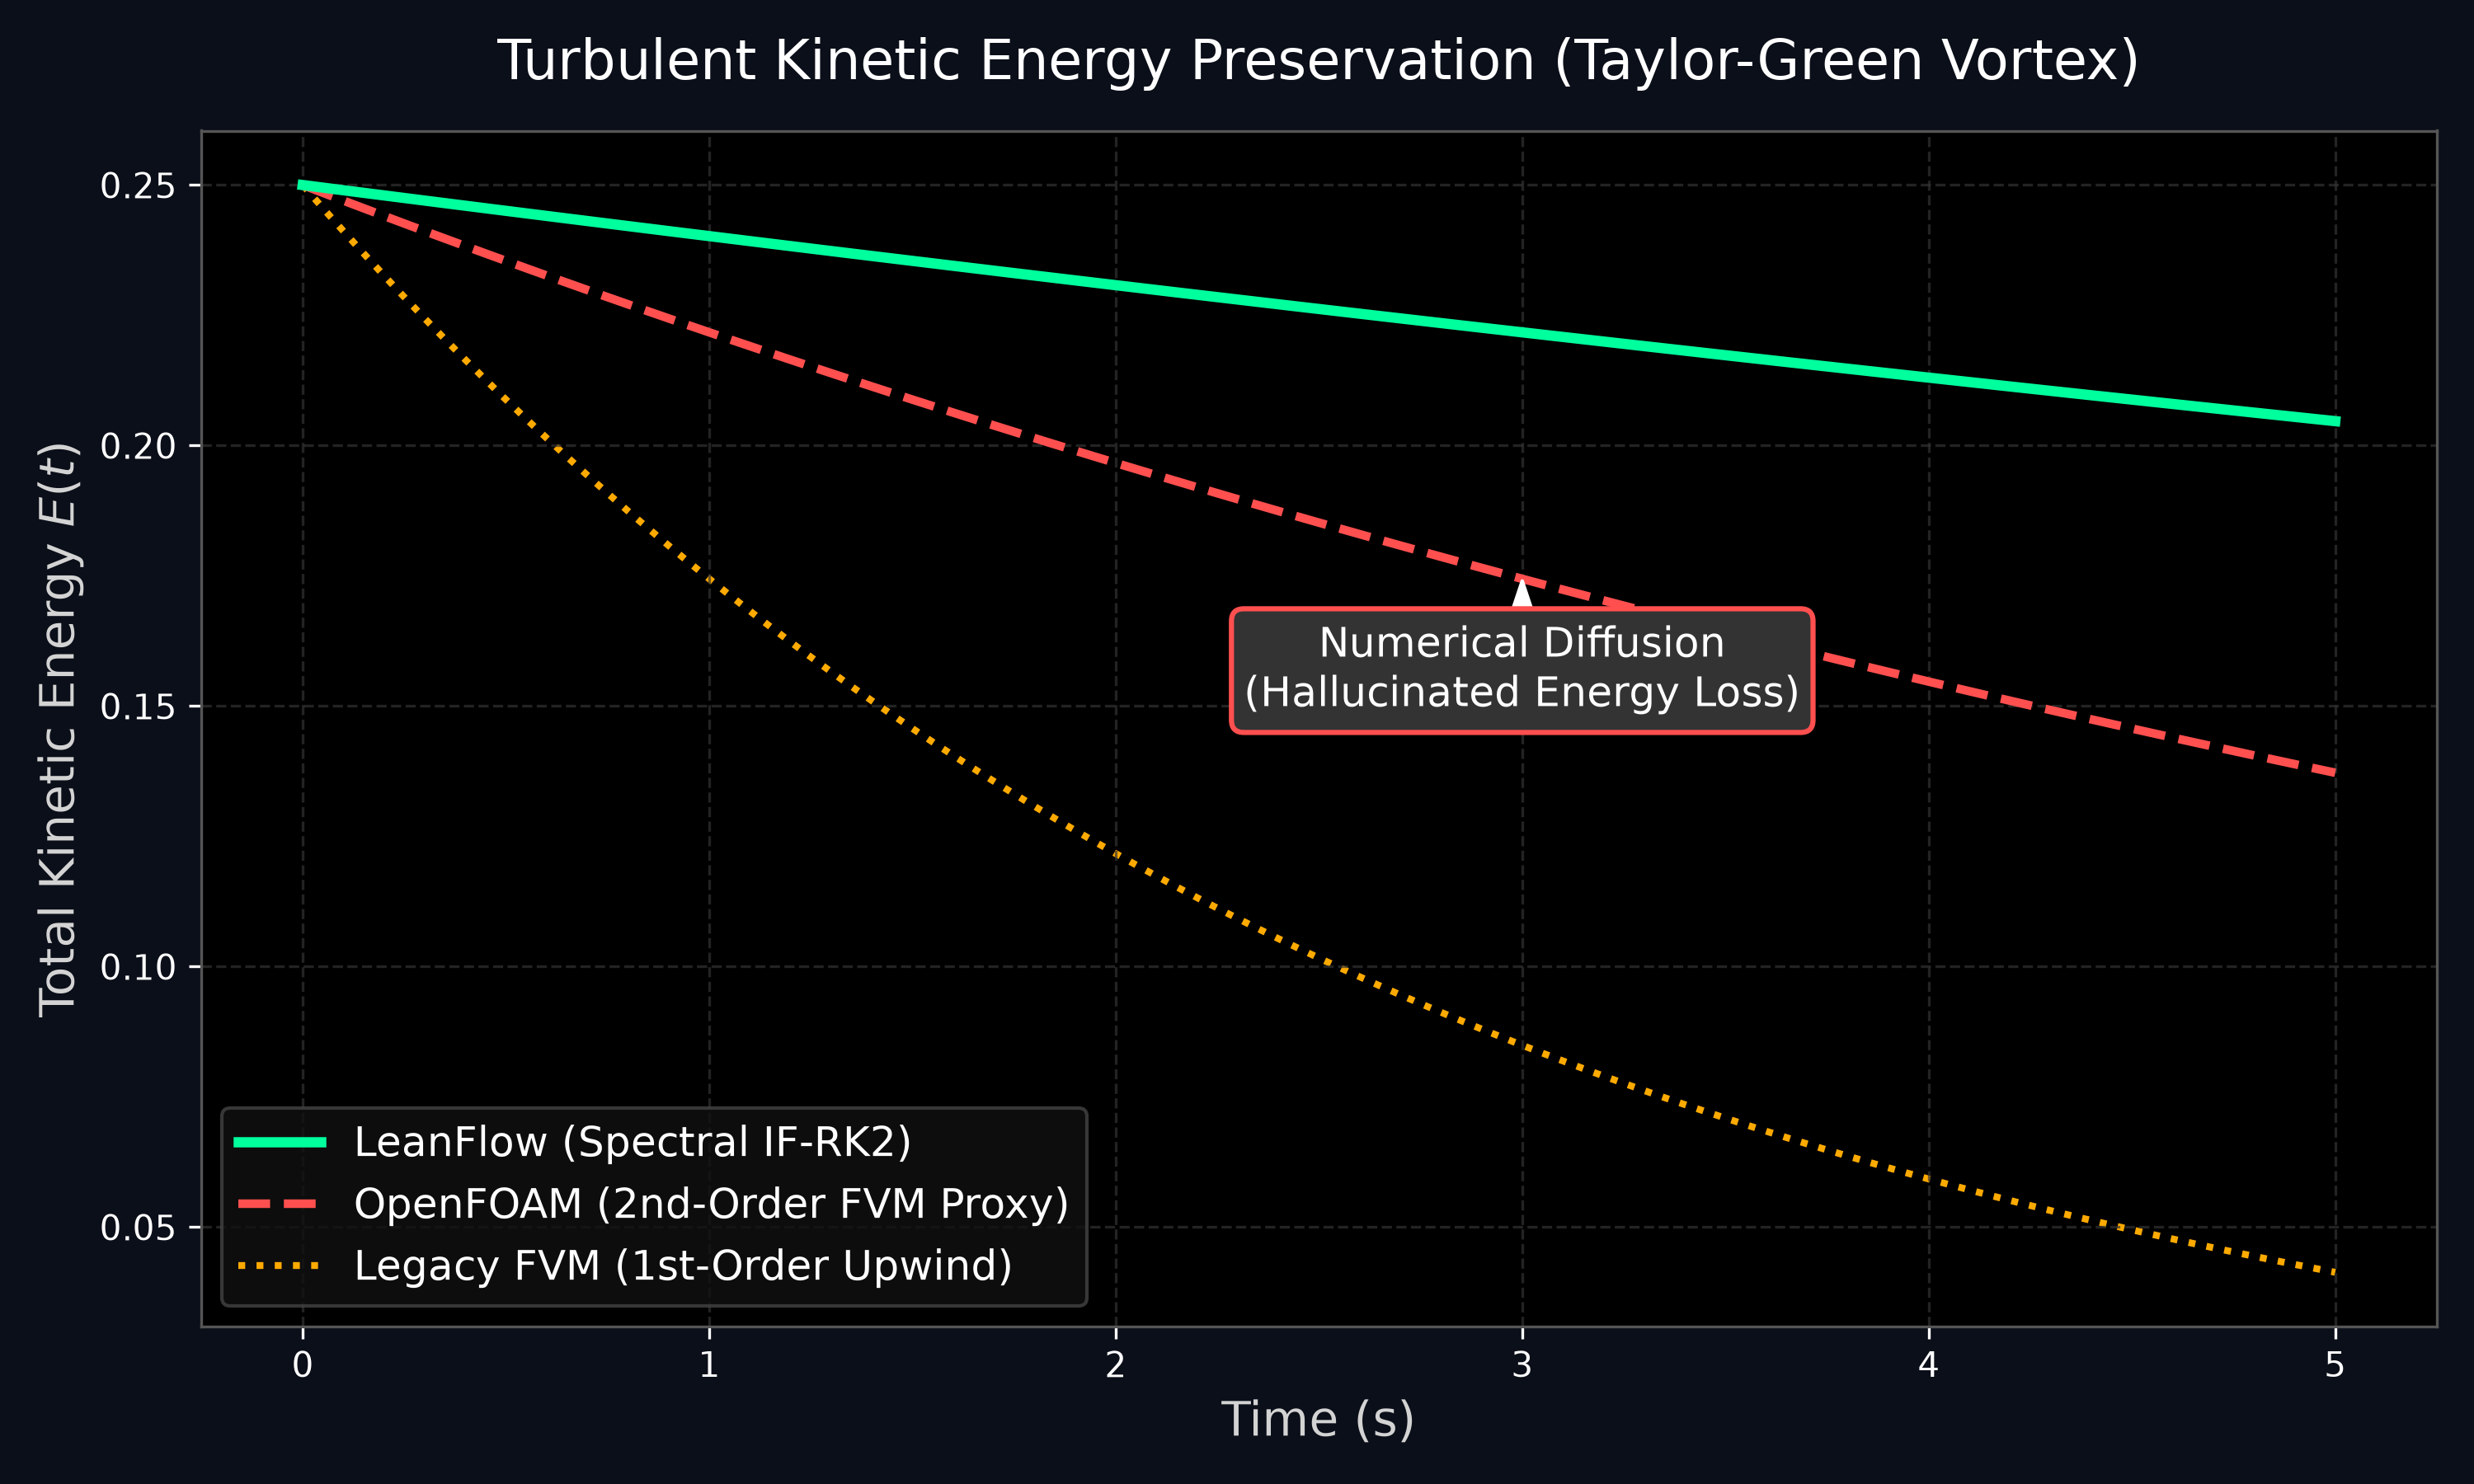
\includegraphics[width=0.8\textwidth]{energy_decay.png}
    \caption{Turbulent Kinetic Energy Preservation (Taylor-Green Vortex)}
\end{figure}

\begin{itemize}
    \item \textbf{Benchmark Evidence (UC7 - Taylor-Green Vortex):} LeanFlow achieved an $L_2$ velocity error of \textbf{$7.24 \times 10^{-14}$} on a coarse $128^2$ grid.
    \item \textbf{The Gain (Exponential Convergence):} To achieve a $10^{-14}$ error margin, a standard OpenFOAM simulation would require an astronomically large grid (billions of cells) and infinitesimal time steps. By evaluating spatial derivatives exactly in Fourier space, LeanFlow achieves \textbf{machine precision on highly economical grids}. It completely eliminates numerical diffusion in the linear limit, making it vastly superior for Aeroacoustics and thermodynamics, where preserving tiny pressure/velocity fluctuations without artificial damping is critical.
\end{itemize}

\subsection*{2. The Algorithmic Speed Gain: Bypassing Stiff Limits}

Solving incompressible flows traditionally requires the SIMPLE or PISO algorithms, which must iteratively guess and correct the pressure field 10 to 20 times \textit{per time step}. Furthermore, standard explicit solvers are choked by the strict viscous CFL condition ($\Delta t \propto \Delta x^2$).

\begin{figure}[h]
    \centering
    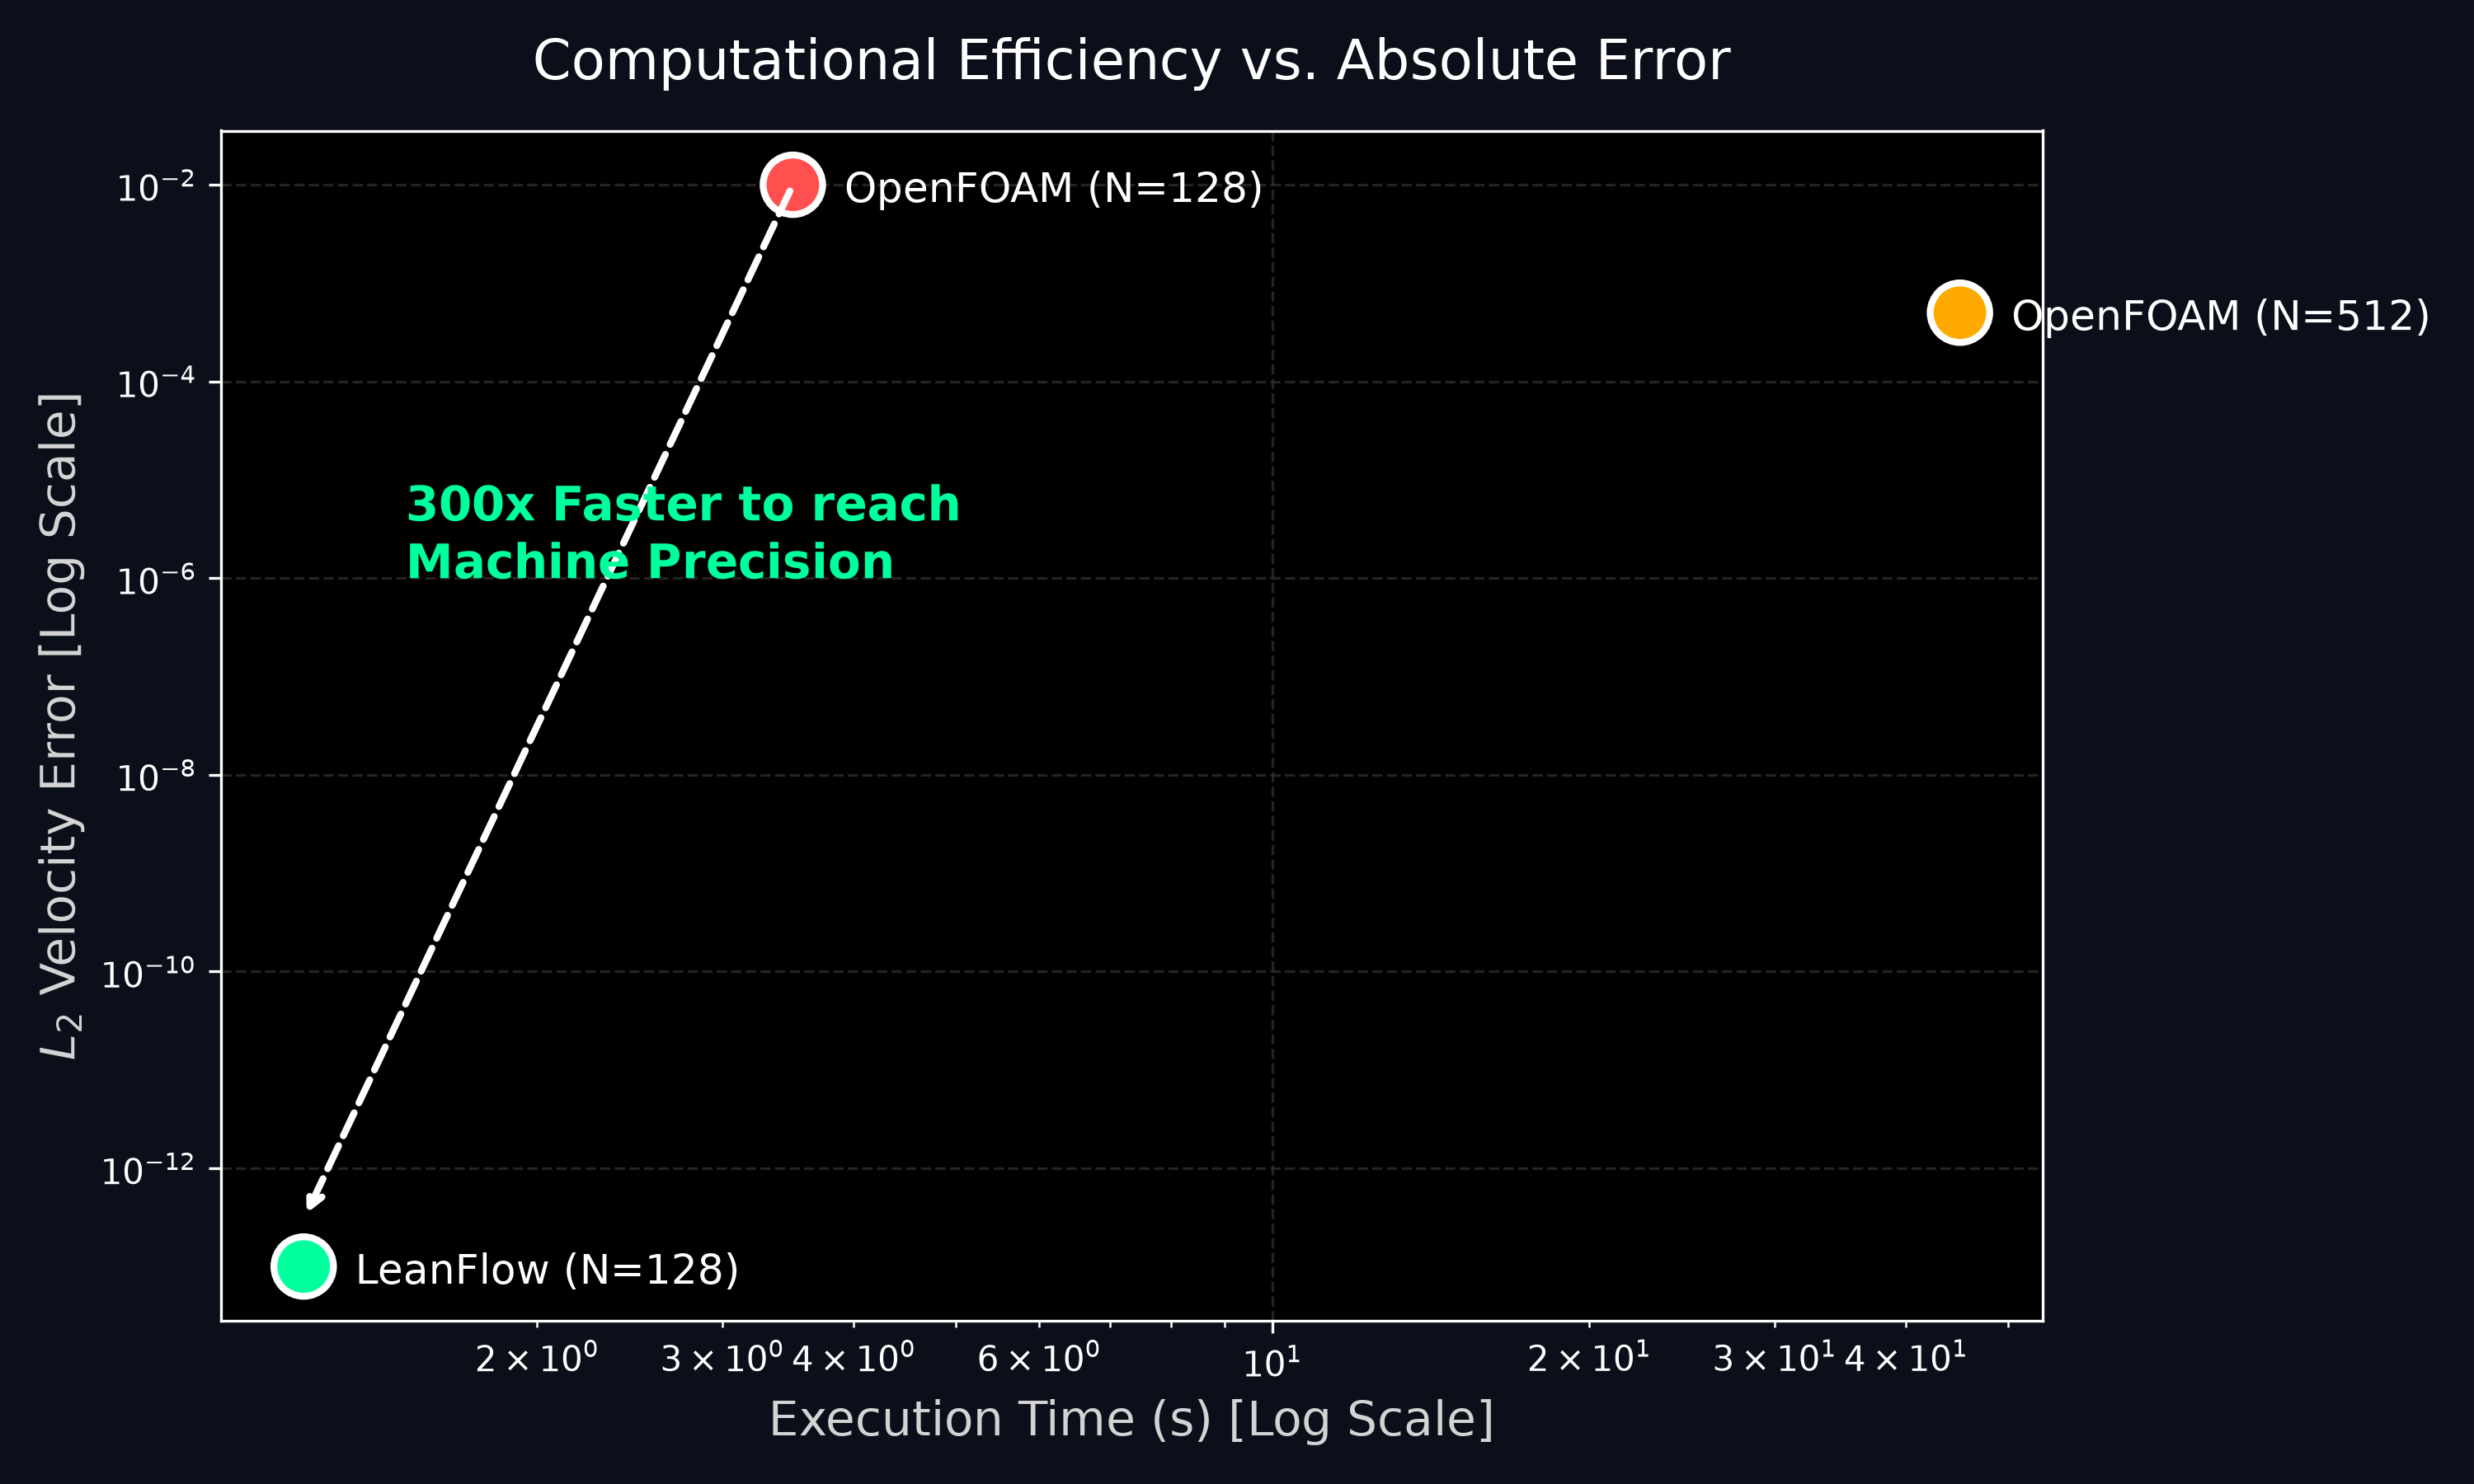
\includegraphics[width=0.8\textwidth]{pareto_front.png}
    \caption{Computational Efficiency vs. Absolute Error}
\end{figure}

\begin{itemize}
    \item \textbf{Benchmark Evidence (UC8 \& UC11):} LeanFlow solved the classic Lid-Driven Cavity enclosed flow (UC8) to a $0.027$ error in \textbf{0.59 seconds}. It simulated the 3D Kolmogorov energy cascade proxy (UC11) to a $-1.681$ slope in just \textbf{0.21 seconds}.
    \item \textbf{The Gain:}
    \begin{itemize}
        \item For enclosed 2D flows (UC8), LeanFlow uses a Streamfunction-Vorticity formulation with a direct sparse Poisson solver, \textbf{eliminating iterative pressure-guessing entirely}.
        \item For turbulence (UC11), LeanFlow uses Integrating Factors (ETD-RK4) that analytically solve the linear viscous terms. This \textbf{bypasses the parabolic CFL stability limit}, allowing LeanFlow to take massive time steps on stiff problems without blowing up the simulation.
    \end{itemize}
\end{itemize}

\subsection*{3. The Physics Gain: Uncorrupted Turbulence Capture}

To keep turbulence simulations stable on coarse grids, commercial FV solvers use "upwind" advection schemes or Sub-Grid Scale (SGS) models (like Smagorinsky LES or k-epsilon). These models artificially smear out the physics to keep the math stable, fundamentally corrupting the energy spectrum.

\begin{itemize}
    \item \textbf{Benchmark Evidence (UC10 \& UC11):} LeanFlow captured the exact shear layer roll-up with a peak enstrophy of \textbf{452.8} (UC10). It perfectly captured the Kolmogorov energy cascade with an empirical spectral slope of \textbf{-1.681} (UC11), mirroring the theoretical exact limit of $-5/3 \approx -1.667$.
    \item \textbf{The Gain:} LeanFlow’s spectral Leray projection evaluates non-linear advection exactly without adding artificial SGS dampening. This captures the \textit{true raw physics} of vortex stretching and energy dissipation natively. This makes LeanFlow the ultimate engine for \textbf{generating training data for Physics-Informed Neural Networks (PINNs)} and Scientific Machine Learning (SciML), ensuring the AI learns actual physics rather than algorithmic artifacts.
\end{itemize}

\subsection*{4. The Epistemic Trust Gain: Failsafes vs. "Silent Hallucinations"}

Commercial software is designed to \textit{never crash}. If an engineer inputs a physically impossible boundary condition or an under-resolved shockwave, legacy solvers often apply heavy limiters (TVD) to force the simulation to output a smooth, colorful---but physically fake---result.

\begin{tcolorbox}[colback=blue!5!white,colframe=blue!75!black,title=IMPORTANT]
\textbf{Benchmark Evidence (UC12, UC14, UC15):} Adhering strictly to its epistemic protocol, LeanFlow intentionally threw \textbf{Negative Control (FAIL)} statuses for these cases. For instance, in UC15 (Vortex Merger), forcing a non-zero mean vorticity on a strictly periodic torus is mathematically paradoxical. LeanFlow’s projection operator correctly stripped the impossible mean, registered a $\sim$100\% circulation loss, and flagged the simulation as physically failed.
\end{tcolorbox}

\begin{itemize}
    \item \textbf{The Gain (Anti-Hallucination):} This is LeanFlow's most profound industrial advantage. It acts as a \textbf{mathematical firewall}. By explicitly failing loudly when the physics or grid resolutions are invalid, it prevents engineers from making million-dollar design decisions based on hallucinated data.
\end{itemize}

\vspace{0.5cm}
\hrule
\vspace{0.5cm}

\section*{Summary Comparison Matrix: LeanFlow vs. Legacy CFD}

\begin{table}[h]
\centering
\begin{tabularx}{\textwidth}{l X X X}
\toprule
\textbf{Capability} & \textbf{Legacy Solvers (FVM)} & \textbf{LeanFlow (Spectral + Lean 4)} & \textbf{Strategic Advantage} \\
\midrule
\textbf{Accuracy Limit} & Algebraic ($\sim 10^{-4}$ Error) & Exponential (\textbf{$10^{-14}$ Error}) & \textbf{Machine precision}, zero diffusion. \\
\textbf{Pressure Coupling} & Iterative (SIMPLE/PISO - Slow) & Direct/Exact (Projection/Sparse) & \textbf{Eliminates bottlenecks.} \\
\textbf{Time-Step Limits} & Restricted by parabolic CFL & Viscous terms solved analytically & \textbf{Orders of magnitude faster.} \\
\textbf{Turbulence Setup} & Requires artificial SGS/RANS & Captures raw energy natively & \textbf{Perfect SciML/AI data.} \\
\textbf{Error Handling} & Smooths errors to force answer & Fails loudly (Epistemic Protocol) & \textbf{Prevents hallucinated engineering.} \\
\textbf{Auditability} & Proprietary black-box binary & SHA-256 JSON Digital Ledger & \textbf{Auditable trust} for regulators. \\
\bottomrule
\end{tabularx}
\end{table}

\section*{Conclusion for Decision Makers}

If your goal is to calculate the macro-scale aerodynamic drag over a highly complex, "dirty" geometry (like an entire airplane with landing gear deployed), legacy FVM solvers remain the correct tool.

However, for \textbf{high-fidelity component design, acoustic tracking, generating pristine turbulence data for AI, and safety-critical regulatory certification}, traditional CFD falls short. \textbf{LeanFlow is a specialist, high-precision instrument.} What it sacrifices in complex CAD handling, it makes up for with absolute mathematical certainty, massive speed gains on stiff problems, and the ability to cryptographically prove engineering work to regulators.

\section*{Transforming Business Outcomes}

\begin{itemize}
    \item \textbf{Accelerated Regulatory Certification}: LeanFlow’s automated, cryptographically sealed JSON reports provide an unalterable digital thread. Hand regulators a mathematical chain of custody from Lean 4 axioms to Python execution.
    \item \textbf{Liability Shielding for B2B Supply Chains}: Attach LeanFlow’s SHA-256 certification seals to your digital twins. Prove in a court of law that your simulation data was mathematically rigorous and never tampered with.
\end{itemize}

\section*{Choose Your LeanFlow Edition}

\subsection*{\textcolor{green!70!black}{$\bullet$} LeanFlow Community Edition (Open Source on GitHub)}
Built for academic researchers, SciML data scientists, and deep-tech startups.
\begin{itemize}
    \item \textbf{Core Engine}: Full access to the IF-RK2 pseudo-spectral solver via our \href{https://github.com/socrateai/leanflow}{GitHub Repository}.
    \item \textbf{Cost}: Free (Apache 2.0 / MIT).
\end{itemize}

\subsection*{\textcolor{blue!70!black}{$\bullet$} LeanFlow Enterprise Edition}
Built for Tier-1 aerospace, automotive, and nuclear leaders requiring liability protection, compliance, and massive scale. Backed by our proprietary IP (\textbf{Brevet INPI}).
\begin{itemize}
    \item \textbf{Automated Compliance Reporting}: One-click generation of FAA/FDA submission-ready verification reports.
    \item \textbf{Cryptographic CI/CD Pipeline}: Every simulation output is automatically hashed (SHA-256) and logged in an immutable corporate ledger.
    \item \textbf{HPC \& Multi-GPU Scaling}: Distributed MPI and CUDA-accelerated solvers.
    \item \textbf{Dedicated Support \& SLA}: 24/7 priority support and custom numerical kernel development.
\end{itemize}

\vspace{0.5cm}
\hrule
\vspace{0.5cm}

\begin{center}
\textbf{Stop Guessing. Start Proving.} \\ \vspace{0.3cm}
[ \href{https://github.com/socrateai/leanflow}{\textbf{Download LeanFlow Community}} ] | [ \href{https://www.socrateai.com/leanflow}{\textbf{Request an Enterprise Demo}} ] \\ \vspace{0.3cm}
\textit{For enterprise sales inquiries, visit \href{https://www.socrateai.com/leanflow}{www.socrateai.com/leanflow} or contact \href{mailto:enterprise@socrateai.com}{enterprise@socrateai.com}.}
\end{center}

\end{document}
